Việc triển khai ở phía backend của ứng dụng sử dụng nền tảng Render như sau:
\newline
Sau khi hoàn tất việc tạo tài khoản hoặc đăng nhập vào Render, chúng ta sẽ tạo một Web Service ở trên nền tảng này:
\begin{figure}[H]
    \centering
    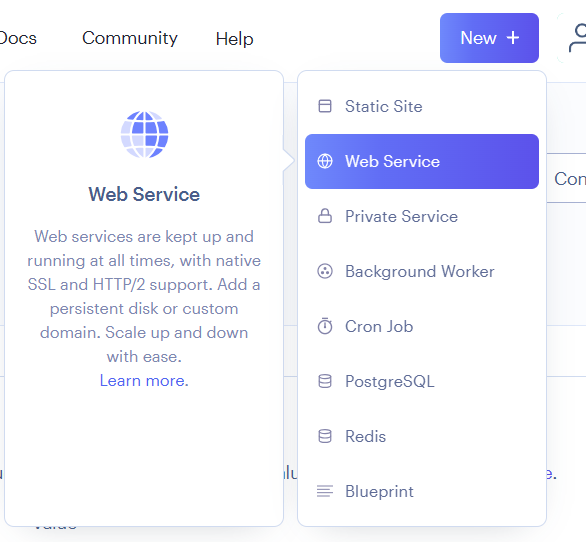
\includegraphics[width=\linewidth]{Content/Hiện thực hệ thống/images/Webservice.png}
    \caption{Giao diện tạo Web service trên Render}
    \label{fig:Tạo Web service}
\end{figure}
Sau đó, ta thiết lập kết nối giữa service trên Render với nơi chứa source code. Ở đây, Render cung cấp 2 lựa chọn là kết nối với Repository trên Github hoặc một Image trên các nền tảng khác. Nhóm chúng tôi lựa chọn phương án đầu tiên.
\begin{figure}[H]
    \centering
    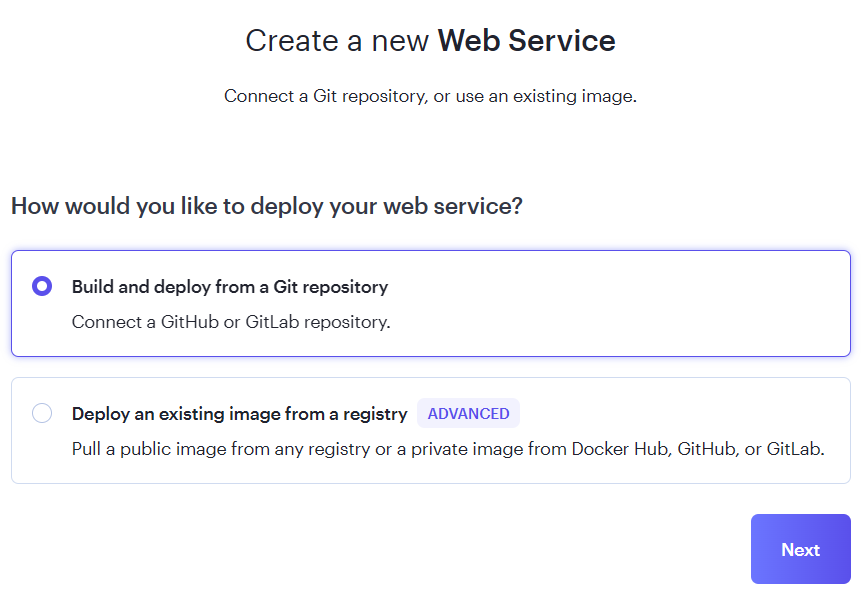
\includegraphics[width=\linewidth]{Content/Hiện thực hệ thống/images/gitrepo.png}
    \caption{Chọn kết nối với Repository}
    \label{fig:Chọn kết nối với Repository}
\end{figure}
Sau đó, chúng ta sẽ chọn kết nối đến một Repository cụ thể. Ở đây, chúng tôi chọn kết nối đến Repository BPE - be tương ứng với phần backend của hệ thống:
\begin{figure}[H]
    \centering
    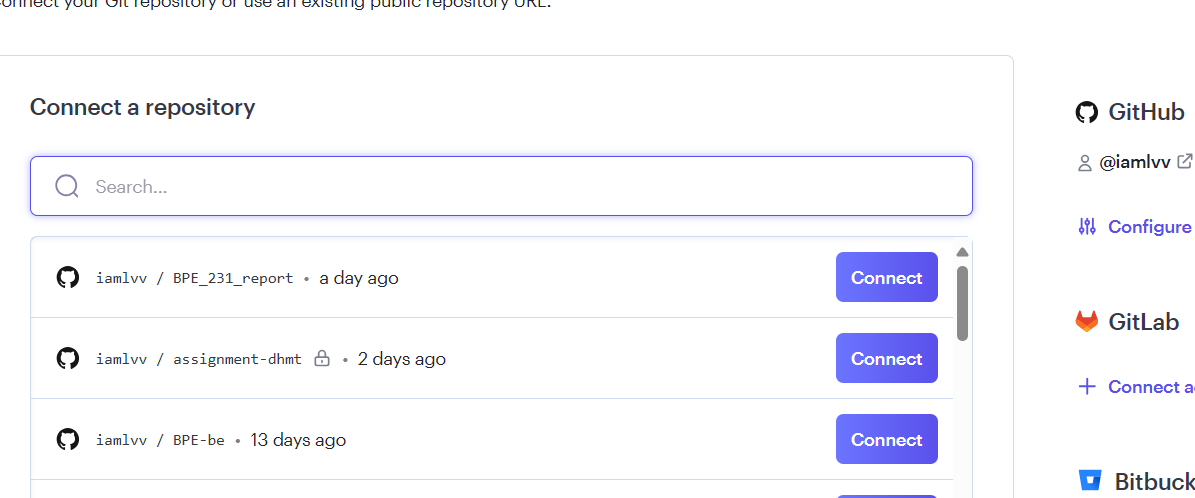
\includegraphics[width=\linewidth]{Content/Hiện thực hệ thống/images/chooserepo.png}
    \caption{Kết nối với Repository của Backend}
    \label{fig:Kết nối với Repository của Backend}
\end{figure}
Sau đó, chúng ta cần điều chỉnh một số những thiết lập để service có thể tự triển khai trên source code của mình. Cụ thể, ta cần chọn nơi đặt server để chạy web service, hay nhánh (branch) trên repository được chọn để triển khai, thiết lập các biến môi trường cũng như câu lệnh để cài đặt các dependencies và khởi chạy server.
\begin{figure}[H]
    \centering
    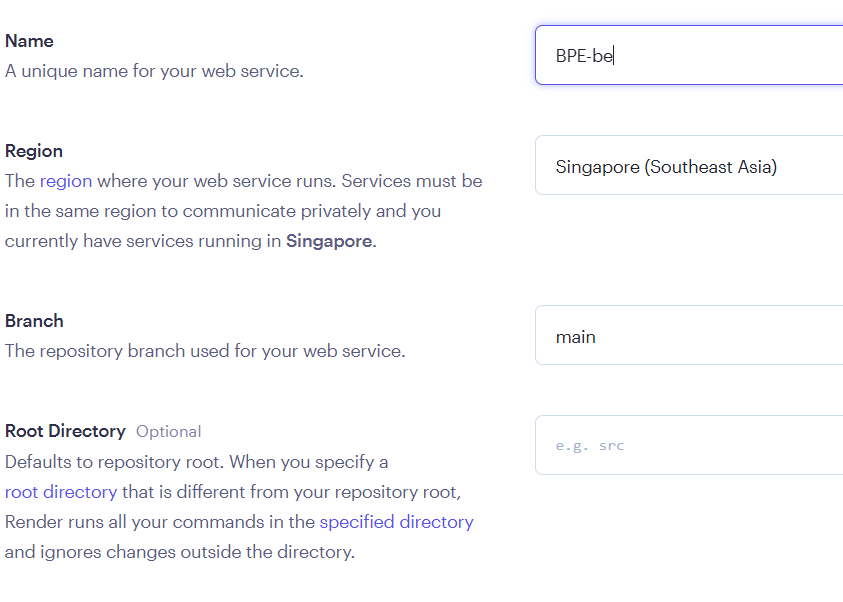
\includegraphics[width=\linewidth]{Content/Hiện thực hệ thống/images/config.png}
    \caption{Thiết lập service}
    \label{fig:Thiết lập service}
\end{figure}
Render cũng cung cấp thêm một số những phiên bản trả phí. Với nhu cầu của chúng tôi đó là một máy chủ luôn trong trạng thái sẵn sàng cho các yêu cầu từ người dùng, và có khả năng lưu trữ file lâu dài, chúng tôi chọn sử dụng phiên bản trả phí Starter - đáp ứng được những nhu cầu trên.
\newline
Như vậy, chúng tôi đã triển khai phần backend của hệ thống lên một PaaS là Render với url \url{https://bpe.onrender.com}. Sau khi triển khai, chúng tôi có thể theo dõi những yêu cầu từ người dùng, cũng như những độ đo khác của hệ thống như băng thông, mức sử dụng CPU, RAM và một số những trạng thái khác.

